 \documentclass[aps,prb,twocolumn,showpacs,superscriptaddress,groupedaddress]{revtex4}

%\usepackage[printfigures]{figcaps}
\usepackage[T1]{fontenc}
\usepackage[english]{babel}
\usepackage{epsfig}
\usepackage{graphicx}
\usepackage{color}
\usepackage{amsmath}
\usepackage{bbold}

\bibliographystyle{plain}

%\newcommand{\bs}[1] {\boldsymbol{#1}}
\newcommand{\bs}[1] {\mathbf{#1}}
\newcommand{\ve}{V}
\newcommand{\fl} [2]{#1^{\Lambda}_{\mathrm{#2} }  }

\begin{document}

\title{Self Energy effect in frequency dependent Vertex flow equation}

\author {D. Vilardi}
\author{C. Taranto}
\author{W. Metzner}
\affiliation{Max Planck Institute for Solid State Research, Stuttgart}

\date{\today}

\begin{abstract}
blablabl ...
\end{abstract}

\pacs{}
\maketitle

\section{Introduction}
\label{sec:introduction}
%The two-particle vertex is an essential building block for the microscopical foundation of the Landau's Fermi-liquid theory \cite{landau1957theory,Landau1958,Pomeranchuk1958} and guarantees the possibility of connecting Fermi-liquid and Renormalization

The formulation of the Wetterich equation\cite{Wetterich1993} laid the basis for a class of powerful new methods that generally go under the name of functional Renormalization Group (fRG).\cite{Metzner2012,Berges2002}
 Given the generality of the Wetterich equation, different conjugations of the fRG are more or less suited to treat different classes of systems. 
For example, while the derivative expansion is most suited for bosonic systems, for fermionic systems on a lattice an expansion into the fields is likely the most sensible choice.
\emph{Is it correct to write this?Are derivative and field expansion mutually exclusive?} 

In the field expansion implementation of the fRG, the two-particle vertex is the core object %in the flow equations and the object%
 to study in order to understand the physical properties of the system. 
However due to its dependence on three frequency and three momentum arguments the two-particle vertex is an extremely difficult object to deal with, unless drastic approximation are made. 
 For fermions on a lattice the momentum-structure of the vertex has been understood while mostly neglecting the vertex frequency-dependence.
%Understanding the momentum structure and its connection with the physical instabilities of a system can be considered a great achievement of  the fRG. 
In particular, the first results have been obtained using the $N$-patch scheme,\cite{Zanchi1996,Halboth2000,Halboth2000b,Honerkamp2001} in which all momenta are treated on the same footing.
Once an understanding was obtained this way, it was possible to tailor more refined treatments of the momentum dependence, like the form factor decomposition, which focuses on the most relevant physics.\cite{Husemann2009,Eberlein2016}
\emph{is there some older reference?}

A comparable understanding is lacking when considering both momentum and frequency dependencies of the vertex.
The very high computational cost and the conceptual difficulty of interpreting data on the imaginary frequency axis did not allow for a frequency treatment comparable to the momentum one.
Indeed in fRG (for lattice models), frequency has been either completely neglected, by assuming a static vertex, or treated in approximate schemes\cite{Husemann2012} which capture part of the physics only.

In the present paper we start filling in this gap, by presenting fully-fledged fRG results with frequency and momentum dependent vertex.
The vertex frequency dependence plays an increasingly important role when the strong coupling regime is approached, as it has been confirmed mostly for impurity models,\cite{Kinza2013,Wentzell2016} or in the dynamical mean field theory\cite{Metzner1989,Georges1992,Georges1996} (and its diagrammatic extensions)\cite{Rohringer2017} framework.\cite{Rohringer2012}
%\cite{Schaefer2013}
Hence a proper treatment of the vertex frequency-dependence is mandatory for methods that aim at the study of the interplay between fluctuations in all the channels in the presence of strong coupling, like DMF$^2$RG.\cite{Taranto2014} 

Our results show the feasibility, and in some respects, the necessity for an improved frequency treatment of the vertex, also at moderate coupling.
A simpler treatment of the frequency dependence was already pursued by Husemann \emph{et al}.~in Ref.~\onlinecite{Husemann2012}, where they have found the emergence of regions in the parameters space characterized by an unusual divergence in the charge channel for finite frequency transfer, which cannot be connected with a phase transition.
 An analysis of the vertex structure in this region will allow us to explain this feature in terms of simple diagrammatic elements. 

Another drawback of a static vertex approximation is that the difficulty in obtaining a frequency dependent self-energy as well its feedback in the flow, unless some further approximation is employed.\cite{Honerkamp2001}
On the contrary, in this work, we have evaluated also the flow equation of the self-energy. 
We will show that the self-energy feedback  affects the results also qualitatively: by preventing the charge channel from diverging. 
This is in contrast with the common belief that the self-energy feedback plays a minor role in the flow.

The paper is structured as follows. In Sec.~\ref{sec:formalism} we will briefly introduce the model under consideration and the basic equations of the fRG in its expansion in the fields.
After discussing in some more detail our treatment for the two-particle vertex  in Sec.~\ref{sec:vertex}, we will move on to the discussion of the main results in Sec.~\ref{sec:results}. Here we start by a stability analysis, then we show the flow evolution and frequency dependence of the vertex. We then consider the charge divergence with a digrammatic explanation, before turning to the analysis of the obtained self-energy. We draw our conclusions in Sec.~\ref{sec:conclusions}. In the Appendix \ref{sec:FlowEquations} we report all the final expression for the vertex flow equations, while in the Appendix \ref{sec:appPairingChannel} we show the frequency dependence also in the pairing channel.

%\begin{itemize}
%\item Much of the weak coupling momentum structure of the vertex (for the fermionic Hubbard model) is know by means of fRG, its frequency structure has been investigated much less. 
%	\item A systematic study keeping into account the full frequency dependence and a physically motivated approximation for the momentum dependence, and including fluctuations in all channels is still lacking.
%\item Our results show the feasibility, and, in some respects, the necessity  of a complete treatment of the frequency dependence of the vertex, whose impact is particularly large in methods that aim at strong coupling.
%\item We will confirm some results already foreseen by \onlinecite{Husemann2012}, who has shown a "forward scattering instability" already with a simpler frequency parametrization.
%\item With the study of the frequency dependence of the vertex we understand the appearance of a \textit{scattering instability}.

%\item The frequency dependent vertex allows to compute a frequency dependent self energy, often neglected in static fRG.   
%\item We will show that the self-energy feedback in the flow equations is essential to guarantee the consistency between vertex and propagators in the flow equations.
%\item even a Fermi-liquid self-energy can qualitatively change the physical results. 
%\end{itemize}

\section{Formalism}
\label{sec:formalism}
\subsection{Flow equations}

\begin{itemize} 
\item General consideration about functional renormalizaton group: 1PI, truncation, 
\item vertex: notation, momentum and energy conservation, spin. Spin symmetry 

\end{itemize}

In the following paragraph we will introduce the functional renormalization group in the implementation that we used, and we will clarify some notational issue about the vertex. 

Generally speaking, the fRG allows to use the renormalization group idea to approach functional integrals. 
This is done by endowing the non-interacting propagator with an additional dependence on a scale parameter $\Lambda$, which generates an exact functional flow equation with known initial conditions. 

We will apply this approach to the effective action, whose expansions into the fields generates the one-particle irreducible (1PI)  functions. By expanding the functional flow equation one obtains a hierarchy of flow equations for the 1PI functions, involving vertexes of arbitrarily  high orders. 
We will restrict ourselves to the level-two truncation by retaining only the two lowest nonvanishing orders in the expansion, i.e., we consider the flow of the (scale dependent) self-energy $\Sigma^\Lambda$ and of the two-particle 1PI vertex $V^\Lambda$, neglecting the effects of higher order vertexes. 
Hence our approach becomes perturbative, and sums up efficiently, although approximately, the so-called parquet-diagrams. 

\subparagraph*{Symmetry considerations} We use the energy and momentum conservation to fix one of the arguments of the arguments of the self energy and of the vertex. 
Furthermore we restrict ourselves to the spin-symmetric phase. 
Hence for the self-energy  we only need to consider one function depending on one frequency-momentum argument: 
\begin{equation}
\Sigma^\Lambda_{\sigma\sigma'}(k)=\Sigma(k)\delta_{\sigma,\sigma'}, 
\end{equation}
where $\sigma = \{\uparrow, \downarrow\} $, and $k=(\nu,\mathbf{k})$, $\nu$ being a Matsubara frequency and $\mathbf{k}$ a momentum in the first Brillouin zone. 

For the notation of the two-particle vertex we refer to Fig. (fig), where $k_i=(\nu_i,\mathbf{k_i})$,
and $k_4=(\nu_1+\nu_2-\nu_3,\mathbf{k_1+k_2-k_3})$ can be omitted. 
Furthermore  SU(2)-symmetry guarantees that the vertex does not vanish only for six spin combinations, pairwaise equal under spin inversion:
$
 V^\Lambda_{\uparrow\uparrow\uparrow\uparrow} = V^\Lambda_{\downarrow\downarrow\downarrow\downarrow}$, 
$  V^\Lambda_{\uparrow\downarrow\uparrow\downarrow} = V^\Lambda_{\downarrow\uparrow\downarrow\uparrow}  $, and
$  V^\Lambda_{\uparrow\downarrow\downarrow\uparrow } = V^\Lambda_{\downarrow\uparrow\uparrow\downarrow}$.   
Finally, due to SU(2) symmetry and crossing relation one has: 
\begin{eqnarray}
\nonumber
V^\Lambda_{\uparrow\uparrow\uparrow\uparrow}(k_1,k_2,k_3) &=& V^\Lambda_{\uparrow\downarrow\uparrow\downarrow}(k_1,k_2,k_3)\\&-& V^\Lambda_{\uparrow\downarrow\uparrow\downarrow}(k_1,k_2,k_1+k_2-k_3), \\ 
V^\Lambda_{\uparrow\downarrow\downarrow\uparrow}(k_1,k_2,k_3)& =& -V^\Lambda_{\uparrow\downarrow\uparrow\downarrow}(k_1,k_2,k_1+k_2-k_3).
\end{eqnarray}
This allows us to consider for the vertex only one function of three arguments:  $V^\Lambda_{\uparrow\downarrow\uparrow\downarrow}(k_1,k_2,k_3)=V^\Lambda(k_1,k_2,k_3)$, all the others spin components being obtained by symmetry. 

With these considerations the flow equation for the self energy reads: 
\begin{equation}
\frac{d}{d \Lambda} \Sigma^\Lambda(k)= -\int_q  S^\Lambda(q)\left[2V^\Lambda(k,q,q) -V^\Lambda(k,q,k)\right], 
\end{equation}
with $q=(\omega,\mathbf{q})$ and $k = (\nu,\mathbf{k})$ and we use the notation  $\int_{q} =T\sum_\omega \int_{\mathbf{q}}$, and $\int_{\mathbf{q}}=\int  \frac{d\mathbf{q}}{4\pi^2}$ is the normalized integral over the first Brillouin zone. 
\begin{equation}
 S^\Lambda=\frac{dG^\Lambda}{d\Lambda}\Bigg|_{\Sigma=\mathrm{const}} 
\end{equation}
  is the single-scale propagator; $G^\Lambda=\left[(G_0^\Lambda)^{-1}-\Sigma^\Lambda\right]^{-1}$ is the full propagator,  $G_0^\Lambda$ is the non-interacting Green's function. 
  
 \begin{widetext} 
The vertex flow equation can be written as: 
\begin{align}
 \frac{d}{d\Lambda}V(k1,k2,k3) =  \fl{\mathcal{T}}{pp}(k_1,k_2,k_3) +  
  \fl{\mathcal{T}}{ph}(k_1,k_2,k_3) + \fl{\mathcal{T}}{phc}(k_1,k_2,k_3),
\end{align} 
where:\footnote{The equation for the particle-particle channel is slightly different from the one usually reported in fRG. This is because we took $\fl{V}{} = \fl{V}{\uparrow \downarrow \uparrow\downarrow}$ instead of $\fl{V}{} = \fl{V}{\uparrow\downarrow\downarrow\uparrow}$.  }
\begin{eqnarray} 
\fl{\mathcal{T}}{pp}(k_1,k_2,k_3) &=&-\frac{1}{2} \int_q \fl{{P}}{}(q,k_1+k_2-q) \Big\{  \fl{V}{}(k_1,k_2,k_1+k_2-q)\fl{V}{}(k_1+k_2-q,q,k_3)   \\ 
\nonumber
&&+  \fl{V}{}(k_1,k_2,q)\fl{V}{}(q,k_1+k_2-q,k_3) \Big\} ; \\  
\fl{\mathcal{T} } {ph}(k_1,k_2,k_3) & =& -\int_q \fl{P}{}(q,k_3-k_1+q)
\Big\{ 2 \fl{V}{}( k_1,k_3-k_1+q,k_3)  \fl{V}{}(q,k_2,k_3-k_1+q) \\
\nonumber
&&- \fl{V}{}( k_1,k_3-k_1+q,q)  \fl{V}{}(q,k_2,k_3-k_1+q) - \fl{V}{}( k_1,k_3-k_1+q,k_3)  \fl{V}{}(k_2,q,k_3-k_1+q) \Big\}; \\
\fl{\mathcal{T}}{phc}(k_1,k_2,k_3) & =& \int_q \fl{P}{}(q,k_2-k_3+q) \fl{V}{}(k_1,k_2-k_3+q,q)
\fl{V}{}(q,k_2,k_3).
\end{eqnarray} 
Here we have defined the quantity:
\begin{align}
\fl{ {P }}{}(q,q') &= G^\Lambda(q)S^\Lambda(q') +G^\Lambda(q')S^\Lambda(q).
\end{align} 




\end{widetext} 
\section{Vertex approximation}
\label{sec:vertex}
%
% Latex file for Vertex approximation
%
%

%For the parametrization of the vertex, we use bosonic exchange frequencies $\OmPP=\nu_1 + \nu_2$,  
%$\OmPH = \nu_2 - \nu_3$ and $\OmPHC = \nu_3 - \nu_1$.
%If not specify otherwise, we use capital letters for bosonic frequency transfer opposite to fermionic ones.

We start by decomposing the vertex as follows:

\begin{widetext}
\begin{align}
\ve^{\Lambda}(k_1,k_2,k_3) = U - \phi^{\Lambda}_{\mathrm{p}}(k_1+k_2,k_1,k_3) + \phi^{\Lambda}_{\mathrm{m}}(k_3-k_1,k_1,k_3)
 + \frac{1}{2}  \phi^{\Lambda}_{\mathrm{m}}(k_2- k_3,k_1,k_2) - \frac{1}{2} \phi^{\Lambda}_{\mathrm{c}}(k_2-k_3,k_1,k_2),
\end{align}
\end{widetext}

where the physical meaning of each $\phi$ channel is defined by its flow equations:

\begin{align}
\dot{\phi}_{\mathrm{p}}^{\Lambda}(q,k_1,k_3) &= -\mathcal{T}^{\Lambda}_{\mathrm{pp}}(k_1,q-k_1,k_3) , \\
\dot{\phi}_{\mathrm{c}}^{\Lambda}(q,k_1,k_2) &= -2\mathcal{T}^{\Lambda}_{\mathrm{ph}}(k_1,k_2,k_2-1) + \mathcal{T}^{\Lambda}_{\mathrm{phc}}(k_1,k_2,q+k_1) , \\
\dot{\phi}_{\mathrm{m}}^{\Lambda}(q,k_1,k_2) &= \mathcal{T}^{\Lambda}_{\mathrm{phc}}(k_1,k_2,q+k_1) .
\end{align}

It should be emphasized that each channel can be associated with a possible instabily of the 
system. $\phi_{\mathrm{p}}$ is associated to a pairing instability, $\phi_{\mathrm{m}}$ to magnetic 
instabilities and $\phi_{\mathrm{c}}$ to charge instabilities.

%We project each channel into a form factor decomposition, starting from the pairing channel:
We address first the momentum dependence. To this end, we introduce a decomposition of the 
unity by means of a set of orthonormal form factors for the two fermionic momenta $\{f_{l}(\bs{k})\}$ obeying 
the completeness relation:

\begin{equation}
 \int_{\bs{k}}  f_{l}(\bs{k}) f_{m}(\bs{k}) = \delta_{l,m}
\end{equation}

We can then project each channel on a subset of form factors whose choice is physically motivated. 
Let us stress that the full form factor expansion is exact but the truncation introduces an approximation.

For the pairing channel we keep only $f_{s}(\bs{k}) = 1$ and $f_d(\bs{k})=\cos{k_x} - \cos{k_y}$:

\begin{equation}
  \phi^{\Lambda}_{\mathrm{p}}(q,k_1,k_3) =
    \mathcal{S}_{\bs{q}}^{\omega,\nu_1,\nu_3} 
    + f_d\left(\frac{\bs{q}}{2}-\bs{k}_1\right) f_d\left(\frac{\bs{q}}{2}-\bs{k}_3\right) \mathcal{D}_{\bs{q}}^{\omega,\nu_1,\nu_3},
\end{equation}
with the shorthand notation $q=(\omega,\bs{Q})$ and $k_i=(\nu_i,\bs{k}_i)$.

The instability in the channel $\mathcal{S}$ is associated to $s$-wave superconductivity, while $\mathcal{D}$ 
is associated to $d$-wave superconductivity.

For the charge and magnetic channels we restrict ourselves to $f_{s}(\bs{k})=1$ only:
\begin{align}
  \phi_{\mathrm{c}}(q,k_1,k_2) &= \mathcal{C}_{\bs{q}}^{\omega,\nu_1,\nu_2}, \\
  \phi_{\mathrm{c}}(q,k_1,k_2) &= \mathcal{M}_{\bs{q}}^{\omega,\nu_1,\nu_2}
\end{align}
corresponding to instabilities in the charge and magnetic channels, respectively. For now on, for notation simplicity we omit 
the $\Lambda$-dependences of channels $\mathcal{S}$, $\mathcal{D}$, $\mathcal{C}$ and $\mathcal{M}$.

Let us stress that for each channel we have used a different frequency notation.
This consists of one frequency corresponding to the frequency transfered in the specific channel 
and two remaining independent frequencies. At finite temperature the frequency transfer, beeing a sum or a difference of 
two fermionic Matsubara frequencies, is a bosonic Matsubara frequency.

\noindent
The choice of the mixed notation is the most natural since the transferred momentum and 
frequency plays a special role in the diagrammatics.
Indeed, on the one hand, it is the only dependence generated in second order perturbation theory and the main dependence in finite 
order perturbation theory. On the other hand, this notation is convenient in the Bethe-Salpeter equations (cite).

In the fRG literature (cite), where the fermionic frequency dependence is neglected the channel functions above are often losely intepreted as 
mediators of bosonic interactions. Such an interpretation is missing in the presence of all frequencies.

Although one expects a leading dependence in the bosonic frequency, 
in particular in the weak coupling regime, we will see that in some case the dependence on fermionic frequencies can become strong and not negligible.

The flow equations for the channels $\mathcal{S}$,  $\mathcal{D}$, $\mathcal{C}$ and $\mathcal{M}$ can be derived from the projection into form factors of eq. (cite):

\begin{equation}
\dot{\mathcal{S}}_{\bs{q}}^{\omega,\nu_1,\nu_3}  = - \int _{\bs{k}_1} \int_{\bs{k}_2} \mathcal{T}_{\mathrm{pp}}(k_1,q-k_1,k_3)
\end{equation}

\begin{equation}
\dot{\mathcal{D}}_{\bs{q}}^{\omega,\nu_1,\nu_3}  = -
\int _{\bs{k}_1} \int_{\bs{k}_2} f_{\frac{\bs{q}}{2} - \bs{k}_1} \mathcal{T}_{\mathrm{pp}}(k_1,q-k_1,k_3) f_{\frac{\bs{q}}{2} - \bs{k}_3}
\end{equation}

\begin{equation}
\dot{\mathcal{C}}_{\bs{q}}^{\omega,\nu_1,\nu_2}  = 
\int _{\bs{k}_1} \int_{\bs{k}_2}  \mathcal{T}_{\mathrm{phc}}(k_1,k_2,q+k_1) -2\mathcal{T}_{\mathrm{ph}}(k_1,k_2,k_2-q) 
\end{equation}

\begin{equation}
\dot{\mathcal{M}}_{\bs{q}}^{\omega,\nu_1,\nu_2}  = 
\int _{\bs{k}_1} \int_{\bs{k}_2}  \mathcal{T}_{\mathrm{phc}}(k_1,k_2,q+k_1)
\end{equation}


\section{Results}
\label{sec:results}
\subsection{Frequency dependence of Vertex}

\begin{itemize}

\item Forward scattering problem seen by Salmhofer

\item Show phase diagram, $\Lambda_{cri}$ vs $x=1-n$, with and without $\Sigma$ 
          (for differenct $t'$)
          
\item Self energy "solve" the problem of charge instability.

\item Suggestion: The charge problem exists also at van Hove filling where, according to the literature, 
           the $\Sigma$ has no effect when Karrasch approximation is taken into account.

\item  Colorplots: Mag and Charge channel

\end{itemize}

While much of the weak coupling momentum structure of the vertex (for the fermionic Hubbard model) is know by means of fRG, its frequency structure has been investigated much less. 
In recent years several results have been obtained for the single impurity Anderson model vertex, both on its own and as essential ingredient for diagrammatic extensions of DMFT. 
Citare: Rohringer, Kinza, Hafermann, Karrasch, Wentzell (and references therein) for the SIAM. Extensions of DMFT: DGA, DF, DMF2RG, Trilex, Quadrilex. 
However a systematic study keeping into account the full frequency dependence and a physically motivated approximation for the momentum dependence, and including fluctuations in all channels is still lacking.

In this persepctive we will present, in the next section, our results obtained by means of fully frequency dependent fRG.
From the methodologic point of view, these results have to be considered as a proof of principle of the feasibility, and in some resepcts of the necessity, of a complete treatment of the frequency dependence of the vertex, with an impact on methods that aim at the study of strong coupling.
From a more physical persepctive we will confirm some results already foreseen by \onlinecite{Husemann2012} with a simpler frequency parametrization. However the study of the frequncy dependence of the verttex will allow us to gain a deeper understanding in these results, in particular the appearance of a \textit{scattering instability}, and a sensitive reduction of the $d$-wave channel. 

Furthermore, a frequency dependent vertex also allows us to compute the frequency dependent self energy, a task that, within fRG, requires heavier approximations whenver one restricts himself to a static vertex.  
We will show that the self-energy feedback in the flow equations is essential to guarantee the consistency between vertex and propagators in the flow equations.
In fact, it turns out that even a Fermi-liquid self-energy can qualitatively change the physical results. 

\paragraph*{Numerical implementation}
We have implemented numerically the flow equations reported in the appendix. 

Due to the different nature of the momentum arguments of self-energy and vertex we have defined two different patching of the irreducible Brillouin zone. 
%The $\phi$-functions depend on a momentum transfer.  
%For the filling and nearest neighbors hopping that we want to describe, the momentum vectors of the most relevant process are $\mathbf{Q}=(0,0)$, important for superconductivity (in the pairing channel) and ferromagnetism (in the magnetic channel); $\mathbf{Q}=(\pi,\pi)$ and its vicinity, relevant for antiferromagnetism and incommensurate antiferromagnetism; the momentum transfer $2k_F$, as defined in Ref.~\onlinecite{Holder2014}, associated to the onset of charge- and spin-density wave instabilities. 
Similarly to what is done in Ref.~\onlinecite{Husemann2009}, the vertex patching describes more accurately the corners around $(0,0)$ and $(\pi,\pi)$, where, for the cases that we will consider, the instability vectors are located.

The situation is completely different for the self-energy, for which the most relevant physics happens in the vicinity of the Fermi surface, at least in the weak coupling regime. Therefore we chose to concentrate the patches along the Fermi surface and in its immediate vicinity, with some further care close to the antinodal points near $(\pi,0)$, relevant for the physics of antiferromagnetism and pseudogap. The representative points are visualized in Fig. (occupation). 

%It is not necessary  that the patching-schemes for vertex and self-energy are connected, but the number of patches used should be roughly of the same order.
In the calculations presented in the following we have used $29$ patches for the vertex and $44$ for the self-energy.

For the practical implementation of the frequency dependence we found convenient to rewrite $\mathcal{S}$, $\mathcal{D}$, $\mathcal{C}$ and $\mathcal{M}$ as function of three bosonic frequencies. 
For each frequency argument we restricted ourselves to at least $40$ positive and $40$ negative Matsubara frequencies. 
We stress that the number of Matsubara frequencies that can be taken into account in the calculation sets the lowest reachable temperature.
  


\subsection{Forward scattering problem}

\begin{itemize}

\item Introduce perpendicular ladder (PL) for charge.

\item Colorplot of charge in PL.

\item Discuss the role of the Bubble at $\boldsymbol{Q}=(0,0)$ and plot it as a function of $\nu$.

\end{itemize}

\subsection{Self energy effects}

\begin{itemize}

\item With self energy feedback, we didn't find any charge instability problem for any parameters range studied.

\item Plot of the Fermi surface based patch scheme.

\item Plot of $\Sigma(i\omega)$ at $\boldsymbol{k}=(\pi,0)$, $\boldsymbol{k}=\boldsymbol{k}_{HS}$ and $\boldsymbol{k}=(\pi/2,\pi/2)$ in frequency space.

\item Plot of $Z_{\boldsymbol{k}}$

\item Plot of occupation with and without $\Sigma$

\end{itemize}

\section{Conclusions}
\label{sec:conclusions}
Conclusions...

\begin{acknowledgments}
We thank  for valuable discussions .... This research was supported by.
\end{acknowledgments}

\section{Appendices}
\label{sec:appendices}
\subsection{Flow equations}
\label{sec:FlowEquations}

We here report the final expression for the flow equations of each channel.
%To simplify the notation from now on  we omit the $\Lambda$ dependencies.
The flow equation for the $s$-wave superconductivity channel $\mathcal{S}$ reads
\begin{equation}
\dot{\mathcal{S}}_{\bs{Q},\Omega}(\nu_1,\nu_3) = 
  \frac{1}{2} \sum_{\nu}{L_\mathrm{s}}^{\Lambda}_{\mathbf{Q},\Omega} (\nu_1,\nu) {P_{\mathrm{s}}}^{\Lambda}_{\bs{Q},\Omega}(\nu) {L_\mathrm{s}}^{\Lambda}_{\mathbf{Q},\Omega} (\nu,\Omega-\nu_3)
+ \frac{1}{2} \sum_{\nu}{L_\mathrm{s}}^{\Lambda}_{\mathbf{Q},\Omega} (\Omega-\nu_1,\nu) {P_{\mathrm{s}}}^{\Lambda}_{\bs{Q},\Omega}(\nu) {L_\mathrm{s}}^{\Lambda}_{\mathbf{Q},\Omega}(\nu,\nu_3),
\end{equation} 	   
with
\begin{equation}
{P_{\mathrm{s}}}^{\Lambda}_{\bs{Q},\Omega}(\omega) = \int_{\bs{p}}  G^{\Lambda}(\bs{p},\omega)S^{\Lambda}(\bs{Q}-\bs{p},\Omega-\omega) + 
G^{\Lambda}(\bs{Q}-\bs{p},\Omega-\omega) S^{\Lambda}(\bs{p},\omega), 
\label{eq:app:P_pp}
\end{equation} 
and: 
\begin{align} 
\label{eq:Lswave}
{L_\mathrm{s}}^{\Lambda}_{\mathbf{Q},\Omega}(\nu_1,\nu_3) = U-\mathcal{S}^{\Lambda}_{\bs{Q},\Omega} (\nu_1,\nu_3)
+ \int_{\bs{p}}  \Big[ \mathcal{M}^{\Lambda}_{\bs{p},\nu_3-\nu_1}(\nu_1,\Omega-\nu_1) + \frac{1}{2} \mathcal{M}_{\bs{p},\Omega-\nu_1-\nu_3}(\nu_1,\Omega-\nu_1) 
- \frac{1}{2} \mathcal{C}^{\Lambda}_{\bs{p},\Omega-\nu_1-\nu_3}(\nu_1,\Omega-\nu_1) \Big]. 
\end{align}	 
The flow equation for the $d$-wave superconductivity channel  $\mathcal{D}$ reads
\begin{equation}
\dot{\mathcal{D}}^{\Lambda}_{\bs{Q},\Omega}(\nu_1,\nu_3) = 
  \frac{1}{2} \sum_{\nu}{L_\mathrm{d}}^{\Lambda}_{\bs{Q},\Omega}(\nu_1,\nu) {P_{\mathrm{d}}}^{\Lambda}_{\bs{Q},\Omega(\nu)} {L_\mathrm{d}}^{\Lambda}_{\bs{Q},\Omega} (\nu,\Omega-\nu_3) 
+ \frac{1}{2} \sum_{\nu}{L_\mathrm{d}}^{\Lambda}_{\bs{Q},\Omega}(\Omega-\nu_1,\nu) {P_{\mathrm{d}}}^{\Lambda}_{\bs{Q},\Omega}(\nu) {L_\mathrm{d}}^{\Lambda}_{\bs{Q},\Omega}(\nu,\nu_3),
\label{eq:dwaveflow}
\end{equation}
with
\begin{equation}
{P_{\mathrm{d}}}^{\Lambda}_{\bs{Q},\Omega}(\omega) = \int_{\bs{p}}  f_{\mathrm{d}}\left(\frac{\bs{Q}}{2}-\bs{p}\right)^2 
\left[ G^{\Lambda}(\bs{p},\omega)S^{\Lambda}(\bs{Q}-\bs{p},\Omega-\omega) +G^{\Lambda}(\bs{Q}-\bs{p},\Omega-\omega)
S^{\Lambda}(\bs{p},\omega) \right], 
\label{eq:app:P_pp}
\end{equation} 
and: 
\begin{align} 
\label{eq:Ldwave}
{L_\mathrm{d}}^{\Lambda}_{\bs{Q},\Omega}(\nu_1,\nu_3) = -\mathcal{D}^{\Lambda}_{\bs{Q},\Omega}(\nu_1,\nu_3) 
+ \frac{1}{2}\int_{\bs{p}} \left(\cos{p_x}+\cos{p_y}\right) \Big[ 
& \mathcal{M}^{\Lambda}_{\bs{p},\nu_3-\nu_1}(\nu_1,\Omega-\nu_1) 
+ \frac{1}{2} \mathcal{M}^{\Lambda}_{\bs{p},\Omega-\nu_1-\nu_3}(\nu_1,\Omega-\nu_1) \\
\nonumber
&- \frac{1}{2} \mathcal{C}^{\Lambda}_{\bs{p},\Omega-\nu_1-\nu_3}(\nu_1,\Omega-\nu_1) \Big].
\end{align}	 
Since $\mathcal{D}$ is generated during the flow by the other channels only, see Eq. (\ref{eq:Ldwave}), it is the most sensitive channel to the frequency approximation made.  
Neglecting the vertex frequency one will likely overestimate $L_{\mathrm{d}}$, as already mentioned in Ref. \onlinecite{Husemann2012}.

The flow equation for the charge channel $\mathcal{C}$ reads
\begin{equation}
\dot{\mathcal{C}}^{\Lambda}_\bs{Q,\Omega}(\nu_1,\nu_2) = \sum_{\nu}{L_\mathrm{c}}^{\Lambda}_{\bs{Q},\Omega} (\nu_1,\nu) P^{\Lambda}_{\bs{Q},\Omega}(\nu) 
{L_\mathrm{c}}^{\Lambda}_{\bs{Q},\Omega} (\nu,\nu_2-\Omega), 
\end{equation} 	   
with
 \begin{align}  
{L_\mathrm{c}}^{\Lambda}_{\bs{Q},\Omega}(\nu_1,\nu_2)=U-&\mathcal{C}^{\Lambda}_{\bs{Q},\Omega}(\nu_1,\nu_2)
+ \int_{\bs{p}} \Big [
- 2 \mathcal{S}^{\Lambda}_{\bs{p},\nu_1+\nu_2}(\nu_1,\nu_2-\Omega) + \mathcal{S}^{\Lambda}_{\bs{p},\nu_1+\nu_2}(\nu_1,\Omega+\nu_1)
\nonumber
\\ &+  [\cos(Q_x)+\cos(Q_y)]\left( \mathcal{D}^{\Lambda}_{\bs{p},\nu_1+\nu_2}(\nu_1,\nu_2-\Omega) -\frac{1}{2} \mathcal{D}^{\Lambda}_{\bs{p},\nu_1+\nu_2}(\nu_1,\Omega+\nu_1) \right)
\nonumber \\ &+ \frac{3}{2} \mathcal{M}^{\Lambda}_{\bs{p},\nu_2-\nu_1-\Omega}(\nu_1,\nu_2)
+ \frac{1}{2} \mathcal{C}_{\bs{p},\nu_2-\nu_1-\Omega}(\nu_1,\nu_2) \Big],
\label{eq:Lc}
\end{align}
while ${P^{\Lambda}}_{\bs{Q},\Omega}(\omega)$ is given in Eq. (\ref{eq:Pph}).
The equation for the magnetic channel is reported in Eq. (\ref{eq:FlowMag}).
The form factor decomposition allows to decouple the momentum integrals, in the calculation of the $L$'s, Eqns. (\ref{eq:Lxph}), (\ref{eq:Lswave}), (\ref{eq:Ldwave}) and (\ref{eq:Lc}), from the frequency summations in the flow equations, hence reducing the numeric effort.   	 
%\begin{equation}
%P_{\mathrm{c},\bs{Q}}^{\Omega;\omega} = \int_{\bs{p}}  G_{\bs{p},\omega}S_{\bs{Q}+\bs{p},\Omega+\omega} +G_{\bs{Q}+\bs{p},\Omega+\omega}
%S_{\bs{p},\omega},
%\end{equation} 
%and:


%The flow for the $\mathcal{M}$ channel read:
%\begin{equation}
%\dot{\mathcal{M}}_\bs{Q}^{\Omega;\nu_1,\nu_2} = \sum_{\nu}{L_\mathrm{m}}^{\Omega; \nu_1,\nu}_{\mathbf{Q}} P_{\mathrm{m},\bs{Q}}^{\Omega,\nu} {L_\mathrm{m}}^{\Omega; \nu,\nu_2-\Omega}_{\mathbf{Q}}, 
%\end{equation} 	   
%with: 
%\begin{equation}
%P_{\mathrm{m},\bs{Q}}^{\Omega;\omega} = \int_{\bs{p}}  G_{\bs{p},\omega}S_{\bs{Q}+\bs{p},\Omega+\omega} +G_{\bs{Q}+\bs{p},\Omega+\omega}
%S_{\bs{p},\omega},
%\end{equation} 
%and: 
%\begin{align} 
%{L_\mathrm{m}}^{\Omega;\nu_1,\nu_2}_{\bs{Q}}=U+\mathcal{M}_{\bs{Q}}^{\Omega;\nu_1,\nu_2} 
%+ \int_{\bs{p}} \Big \{& - \mathcal{S}_{\bs{p}}^{\nu_1+\nu_2;\nu_1,\nu_1+\Omega}  
%-\frac{1}{2} \mathcal{D}_{\bs{p}}^{\nu_1+\nu_2;\nu_1,\nu_1+\Omega}
%[\cos(Q_x)+\cos(Q_y)] + \\
%&\frac{1}{2} \Big[  \mathcal{M}_{\bs{p}}^{\nu_2-\nu_1-\Omega; \nu_1,\nu_2} 
%- \mathcal{C}_{\bs{p}}^{\nu_2-\nu_1-\Omega,\nu_1,\nu_2} \Big] 
%\Big \} 
%\end{align}	 
\subsection{Pairing channel}
\label{sec:appPairingChannel}
%\begin{figure}
%\includegraphics[width=0.60\textwidth]5{images/Phi_color_s_d_wave_SE_fill0_975.png}
%\caption{Frequency dependence of $\mathcal{S}$ (left panel) and %$\mathcal{D}$ (right panel). Here $T=0.08t$, $t'=-0.32t$, $U=4t$ and %$x=0.025$. The transfer momentum and frequency are $\bs{Q}=(0,0)$ %and $\Omega=0$.}
%\label{fig:pairing975}
%\end{figure}
%\begin{figure}
%\includegraphics[width=0.60\textwidth]%{images/Phi_color_s_d_wave_SE_fill0_600.png}
%\caption{Frequency dependence of $\mathcal{S}$ (left panel) and %$\mathcal{D}$ (right panel). Here $T=0.08t$, $t'=-0.32t$, $U=4t$ and %$x=0.4$. The transfer momentum and frequency are $\bs{Q}=(0,0)$ and %$\Omega=0$.}
%\label{fig:pairing600}
%\end{figure}

\begin{figure}[tbh]
 % \begin{center}
    \subfigure[$x=0.025$]{
    \label{fig:pairing975}
    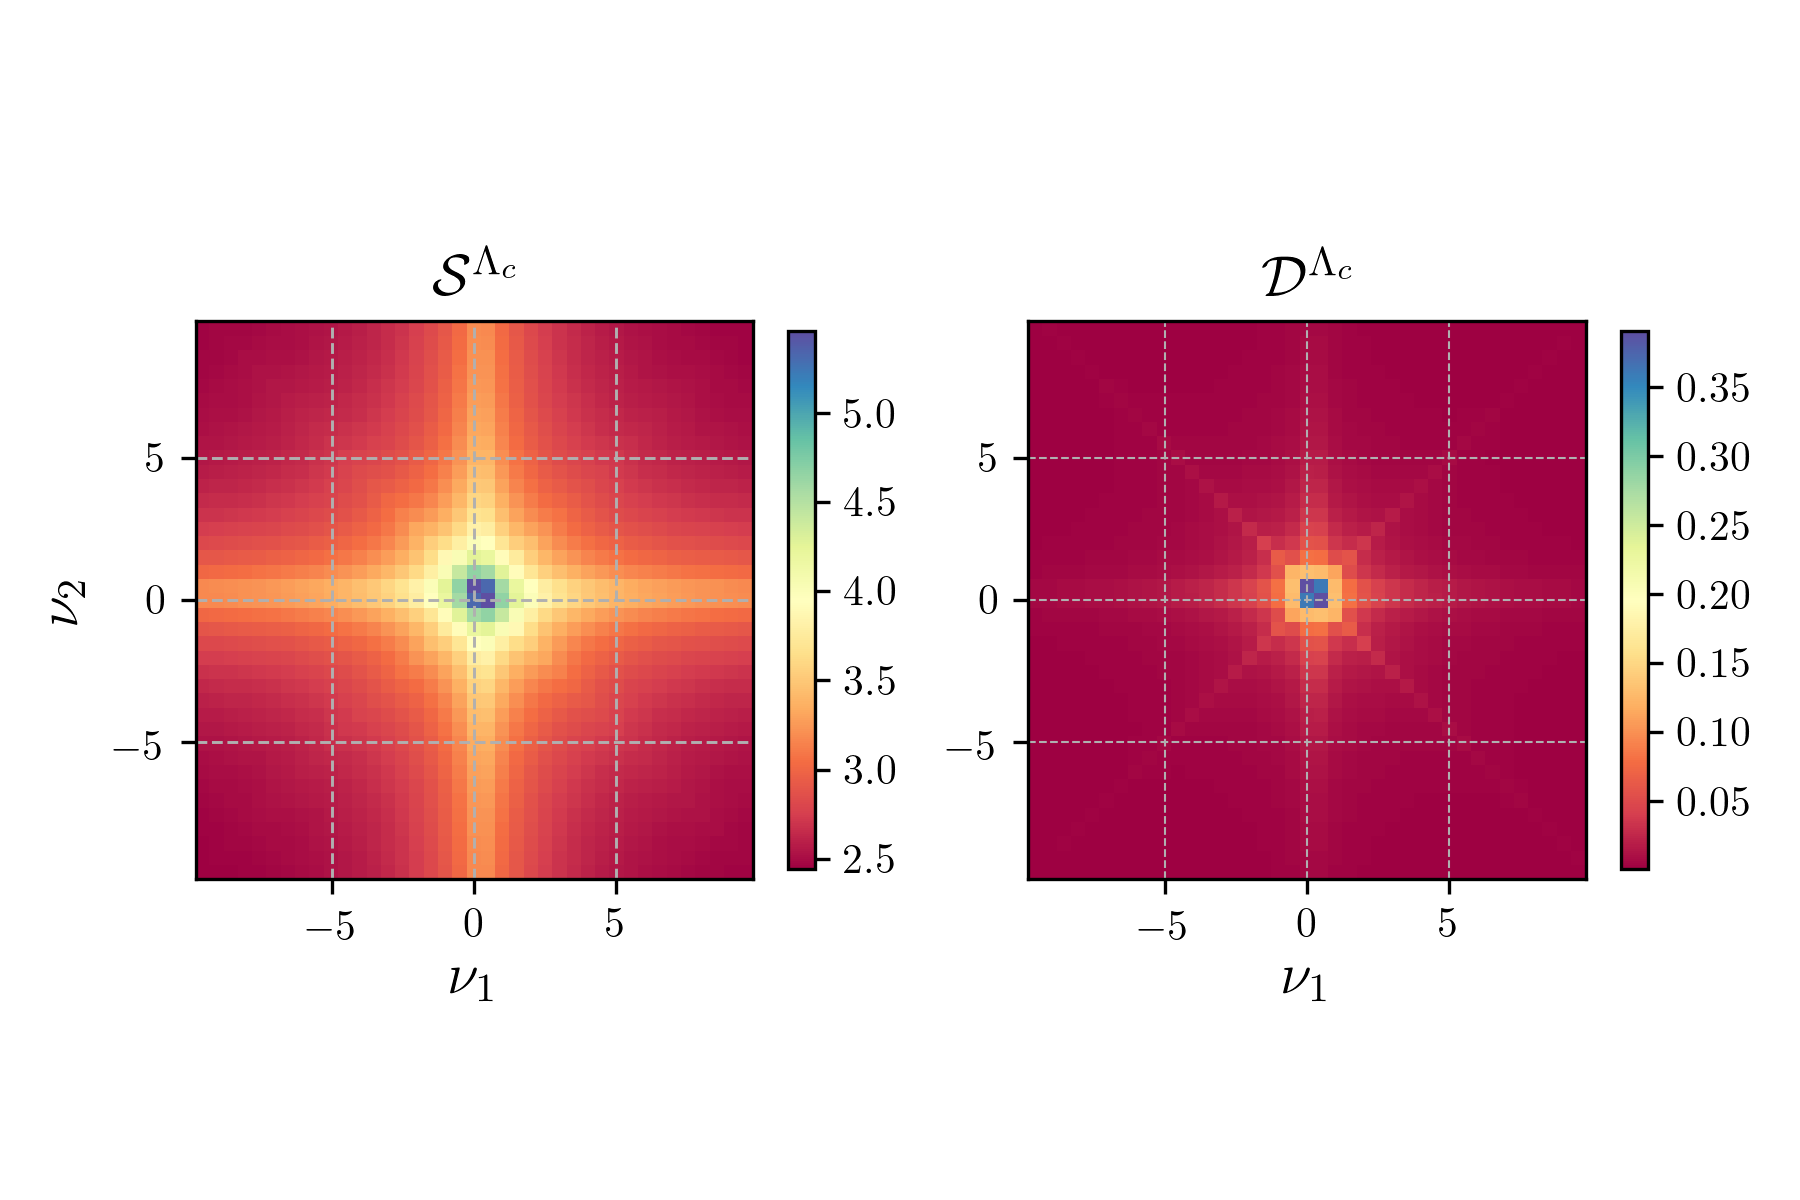
\includegraphics[scale=0.55]{images/Phi_color_s_d_wave_SE_fill0_975.png}}
    \subfigure[$x=0.400$]
    {
    \label{fig:pairing600}
    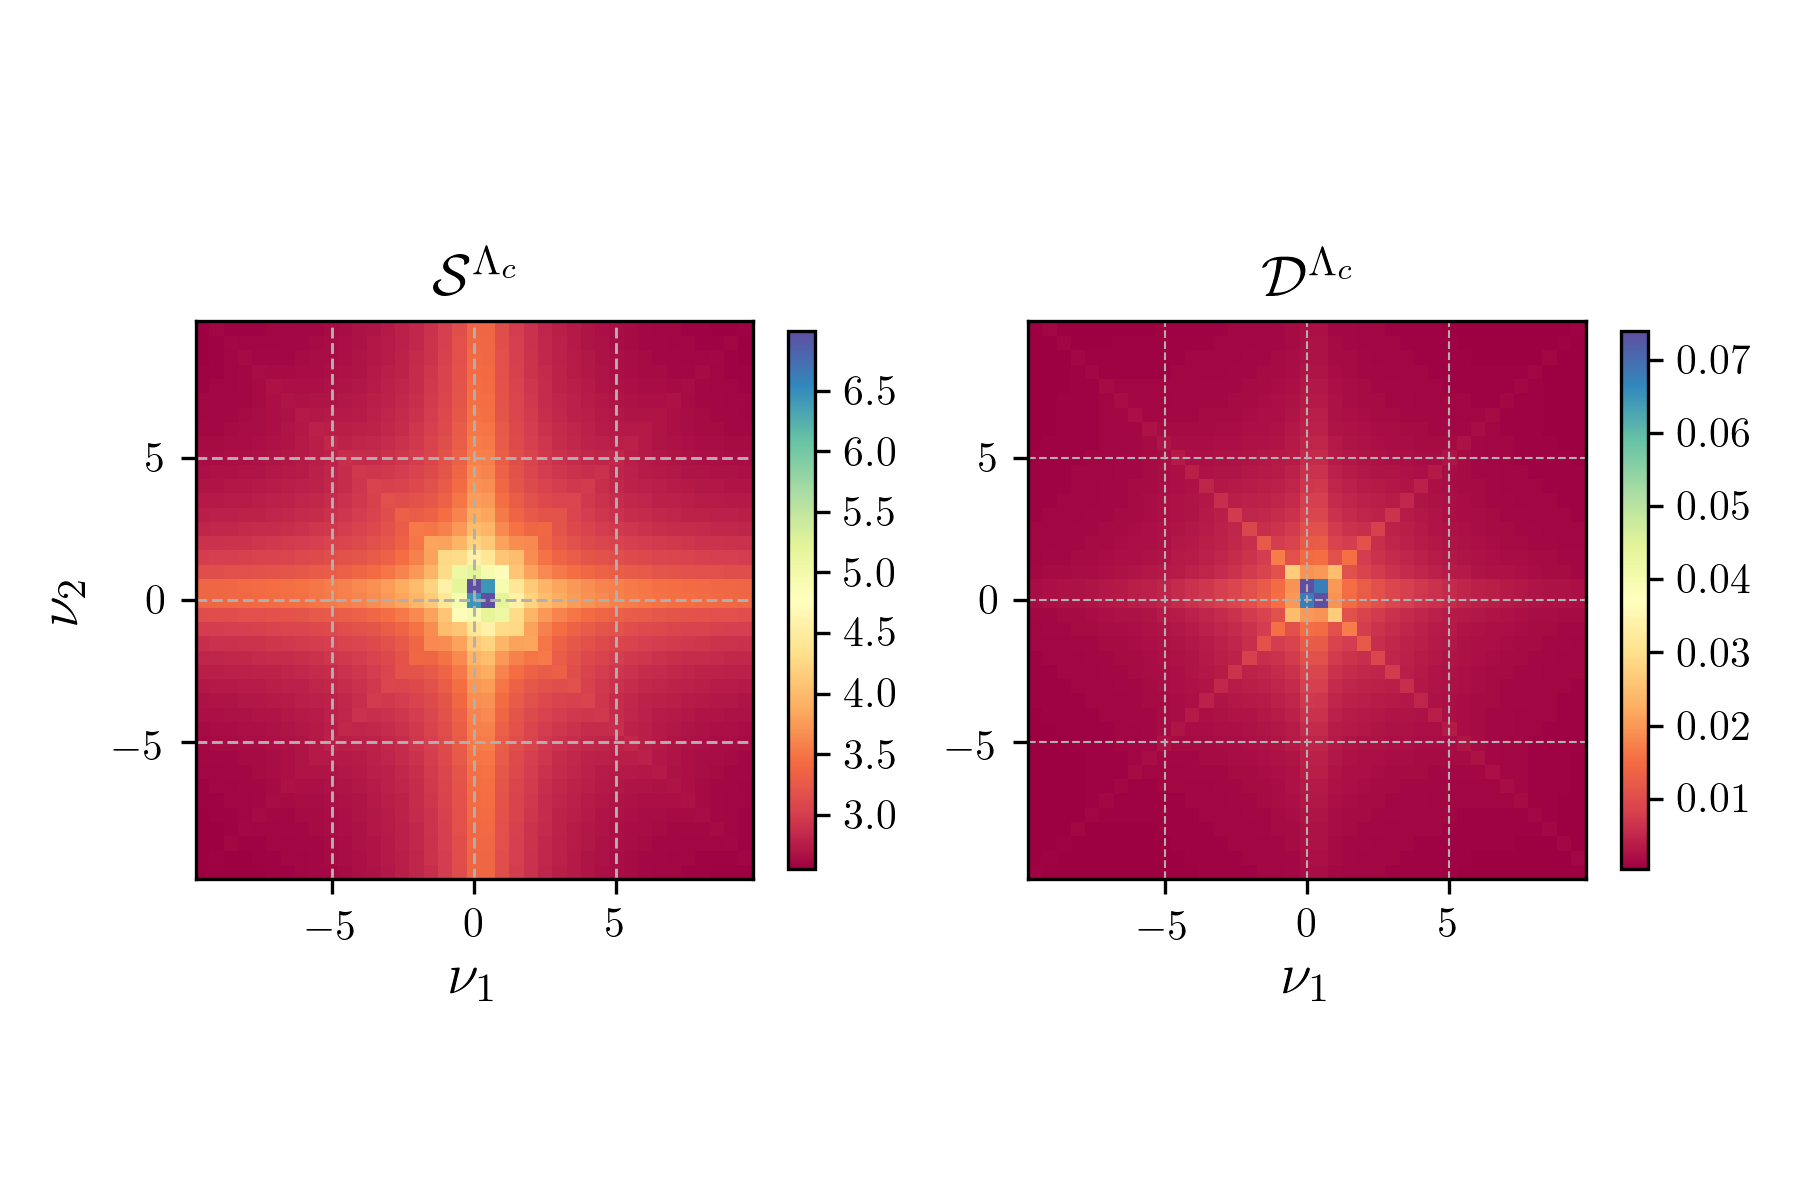
\includegraphics[scale=0.55]{images/Phi_color_s_d_wave_SE_fill0_600.png}} 
 % \end{center}
  \caption{Frequency dependence of $\mathcal{S}$ (left panel) and $\mathcal{D}$ (right panel). Here $T=0.08t$, $t'=-0.32t$, $U=4t$ and $x=0.4$. The transfer momentum and frequency are $\bs{Q}=(0,0)$ and $\Omega=0$.}
  \label{fig:pairing}
\end{figure}




In Fig.~\ref{fig:pairing} we display the frequency dependence of the pairing functions $\mathcal{S}$ and $\mathcal{D}$. 
As a consequence of Eq.~(\ref{eq:Ldwave}) the frequency structure of $\mathcal{D}$ is decaying in all directions.\cite{Wentzell2016a}
The small numerical values are due to three main reasons: 
first, the $d$-wave pairing is expected to increase suddenly for temperatures immediately above its critical temperature. 
Second, as argued in Ref.~\onlinecite{Husemann2012}, previous fRG calculations with a static vertex are likely to overestimate the $d$-wave channel by neglecting the frequency dependence in Eq.~(\ref{eq:Ldwave}). 
Finally, the interaction scheme itself has a tendency to suppress the $d$-wave pairing, since in the terms of Ref.~\onlinecite{Wentzell2016a}, the diagrammatic contributions to $\mathcal{D}$ can be classified as \emph{rest function}.
 


\bibliography{refs}
\bibliographystyle{unsrt}

\end{document}
